\documentclass[10pt,twocolumn,letterpaper]{article}

\usepackage{iccv}
\usepackage{times}
\usepackage{epsfig}
\usepackage{graphicx}
\usepackage{amsmath}
\usepackage{amssymb}
\usepackage{epstopdf}
\usepackage{caption}
\usepackage{subcaption}
\usepackage{enumitem}

\usepackage{xcolor}
\usepackage[breaklinks=true,colorlinks=true,bookmarks=false,pagebackref]{hyperref}

\usepackage{eso-pic, rotating, graphicx}

% Include other packages here, before hyperref.
\usepackage{tikz}

% If you comment hyperref and then uncomment it, you should delete
% egpaper.aux before re-running latex.  (Or just hit 'q' on the first latex
% run, let it finish, and you should be clear).
\usepackage[breaklinks=true,bookmarks=false]{hyperref}

\iccvfinalcopy % *** Uncomment this line for the final submission

\def\iccvPaperID{****} % *** Enter the ICCV Paper ID here
\def\httilde{\mbox{\tt\raisebox{-.5ex}{\symbol{126}}}}

% Pages are numbered in submission mode, and unnumbered in camera-ready
%\ificcvfinal\pagestyle{empty}\fi
\setcounter{page}{1}
\begin{document}

%%%%%%%%% TITLE
\title{Interactive Image Segmentation with GrabCut}

\author{Albert Haque \qquad Fahim Dalvi \\
Computer Science Department, Stanford University\\
{\tt\small \{ahaque,fdalvi\}@cs.stanford.edu}
% For a paper whose authors are all at the same institution,
% omit the following lines up until the closing ``}''.
% Additional authors and addresses can be added with ``\and'',
% just like the second author.
% To save space, use either the email address or home page, not both
}

\maketitle
%\thispagestyle{empty}


%%%%%%%%% ABSTRACT
\begin{abstract}
   In this project, we improve GrabCut for image segmentation by using several optimization techniques. We propose an entropy-based gamma computation using spectral histograms for each image. We then employ a one-time user interaction step to correct for mislabeled alpha maps. Our method demonstrates state-of-the-art performance on the GrabCut dataset, achieving an accuracy of 98.1\% and Jaccard of 90.7\%.
\end{abstract}

\section{Introduction \& Related Work}\label{sec:related_work}

There have been significant past research efforts exploring image segmentation. Initial work done by Shi and Malik \cite{shimalik97} used the idea of normalized graph cuts to segment a given image. They provided an approximate solution to the problem of graph partitioning which could be applied to a graph with nodes representing pixels in an image, and the edges representing the similarity between an two given nodes. Boykov and Jolly \cite{boykovjolly01} then introduced another idea in which a user provides ``seeds" to indicate regions containing objects or spanning the background. They use these seeds as hard constraints, while introducing softer constraints between the nodes. They then find the optimal solution using the max flow algorithm. Grabcut is heavily based on this technique. Felzenszwalb et al. \cite{felzenszwalb04} further build upon this idea of representing images as graphs to solve the problem where there is high variability in a given component of the image. They introduce the idea of coarseness to formally distinguish between good and bad segmentations. Another contribution of their paper was the greedy approach they defined, as it was significantly faster than the older approaches, like the one by Shi and Malik \cite{shimalik97}.

\begin{figure}[t]
% Should always be on first page
\centering
\includegraphics[width=1\linewidth]{figures/pull.eps}
\caption{Our Approach. We optimize gamma using the Shannon-entropy of the spectral histogram. Combined with a one-step user interaction step, we achieve state-of-the-art results.}
\label{fig:pull}
\end{figure}

Lempitsky et al. \cite{lempitsky09} introduced a prior on the bounding box prior from  Grabcut. They proposed that a bounding box can provide more information than just marking the pixels outside the bounding box as background. They defined a notion of tightness so that the process does not result in excessively small segmentations. They ensure that the bounding box ``tightly" surrounds their resultant segmentations. Extending Grabcut with this results in a lower segmentation error.

Additional work was done by the authors in \cite{joulin10} to push image segmentation towards an unsupervised task. One idea, introduced by Joulin \etal, used multiple images of the same object to perform automatic segmentation. They used similarity between pixels across two images to define their energy. For example, they look at spatial similarity and discriminative agreement to decide if two pixels (one from each image) belong to the same object. They also provide an optimization solution to minimize the defined energy and achieve a good segmentation.

Finally, Guillaumin et al. \cite{guillaumin2014} introduced the idea of using semantic similarity between images to help with segmentation. Using a segmented source image and a semantically similar target image (i.e. containing a similar object) to transfer the segmentation from the source image and obtain a segmentation for the target image. They use ImageNet, a collection of images grouped together by their semantic similarity.

\section{GrabCut}\label{sec:grabcut}
\subsection{Algorithm}
The Grabcut algorithm by Rother et al. \cite{rother2004grabcut} builds upon the idea presented by Shi and Malik \cite{shimalik97}. It uses a similar graph structure, where each node represents a pixel. Each node is connect to the nodes representing its pixel neighbors, and also to a foreground and background node. The idea is that after performing mincut on the graph, the nodes connected to the foreground node will indicate the pixels in the foreground, and the nodes connected to the background node will indicate the pixels in the background.

The crux of the algorithm lies in the way the weights of the edges are assigned, as that is the information that the mincut algorithm uses to partition the image graph. For the rest of the discussion, we will consider \emph{unary} weights to be the weights of the edges from each node to the foreground/background node, and \emph{pairwise} weights to be the weights on the edges connecting neighboring pixels. 

The model described by Rother et al. uses Gaussian Mixture Models to represent the color space in the images. We have two GMMs in play, one that represents the foreground and one that represents the background. The number of components in each GMM is set such that the variability in the foreground/background can be captured appropriately. For example, if the background is composed of two colors, yellow and red, one component of the GMM would fit on the yellow pixels, while the other one will fit on the red. To initialize these GMMs, we basically use some form of clustering. In the case of our implementation, we decided to use K-means, as it is relatively fast and clusters similar colors into a single component. We also use a fixed number of gaussian components, namely five, as this seems to work well on a vast number of images.

We first use the bounding box supplied by the user to set our initial guess for the foreground and background pixels. Everything inside the bounding box is considered to be foreground, and everything outside it is marked as background. As mentioned earlier, we run K-means on this initial segmentation to construct the GMMs.

\begin{figure}[!t]
\resizebox {\columnwidth} {!} {
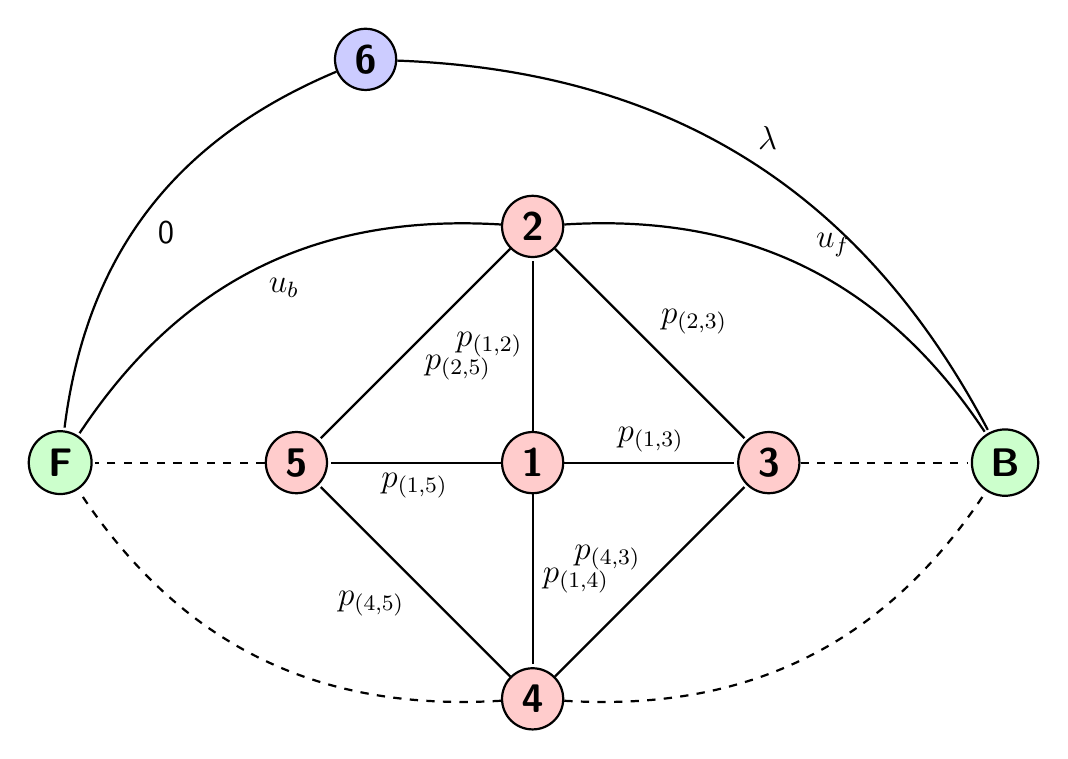
\begin{tikzpicture}[shorten >=1pt,auto,node distance=3cm,
  thick,main node/.style={circle,fill=blue!20,draw,font=\sffamily\Large\bfseries}]
  
    \tikzstyle{foreground} = [circle,fill=red!20,draw,font=\sffamily\Large\bfseries]
    \tikzstyle{background} = [circle,fill=blue!20,draw,font=\sffamily\Large\bfseries]
    \tikzstyle{special} = [circle,fill=green!20,draw,font=\sffamily\Large\bfseries]

  \node[foreground] (1) {1};
  \node[foreground] (2) [above of=1] {2};
  \node[foreground] (3) [right of=1] {3};
  \node[foreground] (4) [below of=1] {4};
  \node[foreground] (5) [left of=1] {5};
  
  \node[special] (6) [left of=5] {F};
  \node[special] (7) [right of=3] {B};
  
  \node[background] (8) [above left of=2] {6};
  
  \path[every node/.style={font=\sffamily\large}]
    (1) edge node {$p_{(1,4)}$} (4)
    (1) edge node {$p_{(1,3)}$} (3)
    (1) edge node {$p_{(1,2)}$} (2)
    (1) edge node {$p_{(1,5)}$} (5)
    (2) edge node {$p_{(2,5)}$} (5)
    (2) edge node {$p_{(2,3)}$} (3)
    (4) edge node {$p_{(4,5)}$} (5)
    (4) edge node {$p_{(4,3)}$} (3)
    
    (2) edge [bend right] node {$u_b$} (6)
    (2) edge [bend left] node {$u_f$} (7)
    
    (8) edge [bend right] node {0} (6)
    (8) edge [bend left] node {$\lambda$} (7)
    
    (4) edge [bend left, dashed] node {} (6)
    (4) edge [bend right, dashed] node {} (7)
    (3) edge [dashed] node {} (7)
    (5) edge [dashed] node {} (6)
    
    ;
    
\end{tikzpicture}
}
\caption{Simplified illustration of GrabCut's internal graph representation. Red nodes indicate pixels inside the bounding box. Blue nodes represent a pixel outside the bounding box (i.e. definitely background). Green nodes represent special foreground and background nodes respectively (i.e. source and sink).}
\label{fig:sample-graph}
\end{figure}

The algorithm then goes through an iterative process of improving the segmentation.  We first assign each pixel a component from the background and the foreground GMM. This is done by simply checking which gaussian component in each of the GMMs retursns the highest probability for any given pixel. Next, using our current segmentation (from the previous iteration, or from the bounding box for the first iteration) we recompute the parameters of each GMM. Basically, we take all the pixels currently segmented as foreground and update the mean and covariance of the foreground GMM, and similarly we use the background pixels for the background GMM. We then assign the weights to the edges of the graph as follows: The unary weights come from each of the gaussian. They are computed as the negative of the log probability of a pixel belonging to the GMM. To reduce computational overhead, the paper suggests that we compute the probability of only the assigned component for every pixel. Let $u_f$ represent the weight from the foreground GMM and $u_b$ represent the weight from the background GMM. The pairwise weights, $p_{(i,j)}$ are computed from the difference between the two pixels. Specifically, $p_{(i,j)} = \gamma \exp{-\beta\|z_i - z_j\|^2}$, where $z_i$ and $z_j$ represent the pixel indexed by $i$ and $j$. $\gamma$ here is set to $50$ from empirical observations, while $\beta$ is computed from the expected difference between pairs of pixels from the image. Note that a higher similarity between the nodes would result in a bigger pairwise term. The example graph in \ref{fig:sample-graph} shows how the weights are set for each node:

Notice that not all edges are shown in the graph for clarity. For the nodes that are inside the bounding box (red nodes), we assign the unary term from the foreground GMM to the edge between a node and the background node, and the unary term from the background GMM is assigned to the edge between a node and the foreground term. The reasoning behind this is that since the unary terms are negative log probabilities, a lower value indicates a higher probability. Therefore, if the node has a higher probability of being in the background (i.e. a higher probability from the background GMM), $u_b$ would be lower, and the mincut algorithm would cut the edge weighted $u_b$, thus partitioning the node with the background node. For the nodes outside the bounding box (blue nodes), we assign 0 weight to the edge to the foreground node, and $\lambda$ weight to the edge to the background node. The idea is to set $\lambda$ to a very high value so that the edge weighted 0 is always cut, and the node is always assigned as background. 

The pairwise terms propagate the information given by the unary terms. For example, if we know a node is definitely background, and a neighboring node is connected with a high pairwise weight, we would like the mincut algorithm to not cut this edge, as the neighbor is probably a part of the background. 

We then run mincut on this graph, and use the resulting partition to assign each pixel to either the foreground or the background, and re-iterate to get a better segmentation.


% Is your implementation exactly the same as the algorithm
% described in the paper? If they are not exactly the same, why
% did you make those changes? The reason might be that you
% think they lead to better performance or one component of
% the original algorithm is very complicated and difficult to
% implement, so you used a simpler approach. Did you make
% any extension to the original algorithm?  How did you set
% any parameters used in the code? Were any implementation
%details missing in the original paper, and if so, how did you
% address this problem?

\subsection{Extensions}
Extensions we did including gamma optimization, user interaction, and hyperparameter tuning. Results for each extension are shown in Section \ref{sec:experiment}.
\subsubsection{Hyperparameter Tuning}
To further improve results, we tuned several GrabCut hyperparameters and show their results in Section \ref{sec:experiment}:
\begin{enumerate}[topsep=4pt,itemsep=0ex,partopsep=1ex,parsep=0.5ex]
\item Number of iterations
\item Number of GMM components, $K$
\item Neighborhood size
\end{enumerate}
We adopt a grid-search approach and do not modify the original GrabCut implementation for this extension.

\subsubsection{Tight versus Loose Bounding Box}
A tighter bounding box not only gives us more pixels that can be marked as definitely background, but also gives our background GMM more information to learn from. Hence, we decided to extract tight bounding boxes from the given ground truth segmentations and run our grabcut algorithm on these bounding boxes.

\subsubsection{User Interaction for Alpha Map}

Color-skewed images presents an interesting challenge: how do you separate the background from the foreground if they are the same color? To address this, we employ a single user interaction step. After five iterations, we show the current segmentation to the user and prompt them to draw lines on the foreground, whose pixels actually belong the the background. This is illustrated in Figure \ref{fig:user_interaction}.

\begin{figure}[t]
\centering
\begin{subfigure}[b]{0.48\linewidth}
        \includegraphics[width=1.0\linewidth]{figures/banana1_ui1.png}
        \caption{After 5 iterations}
\end{subfigure}%
~
\begin{subfigure}[b]{0.48\linewidth}
        \includegraphics[width=1.0\linewidth]{figures/banana1_ui2.png}
        \caption{After 10 iterations}
\end{subfigure}%
\vspace{-2mm}
\caption{Illustration of two user interaction steps}
\label{fig:user_interaction}
\end{figure}

Using this new information, we treat it as ground truth and permanently assign the user selected pixels to the background. The alpha trimap is updated and GrabCut continues the iterative minimization step.

\begin{figure*}[t]
\centering
\begin{subfigure}[b]{0.24\textwidth}
    \includegraphics[width=\textwidth]{figures/experiments/tuning/iterations_accuracy.eps}
    \caption{Iterations (Accuracy)}
    \label{fig:iterations_accuracy}
\end{subfigure}%
~
\begin{subfigure}[b]{0.24\textwidth}
    \includegraphics[width=\textwidth]{figures/experiments/tuning/iterations_jaccard.eps}
    \caption{Iterations (Jaccard)}
    \label{fig:iterations_jaccard}
\end{subfigure}%
~
\begin{subfigure}[b]{0.24\textwidth}
    \includegraphics[width=\textwidth]{figures/experiments/tuning/components_accuracy.eps}
    \caption{Components (Accuracy)}
    \label{fig:components_accuracy}
\end{subfigure}%
~
\begin{subfigure}[b]{0.24\textwidth}
    \includegraphics[width=\textwidth]{figures/experiments/tuning/components_jaccard.eps}
    \caption{Components (Jaccard)}
    \label{fig:components_jaccard}
\end{subfigure}
\caption{Hyperparameter tuning results. We experimented with the number of iterations, number of components, neighborhood size, and bounding box. We use 10 iterations, 10 components, a neighborhood size of four, and a loose bounding box (except when tuning a specific parameter).}
\end{figure*}

\subsubsection{Entropy-Based Gamma Optimization}

We further address the color-skew problem by employing an entropy-based gamma optimization technique. The motivation is that unary energies capture color information better than the pairwise terms. Pixels with a similar color will have a small pairwise term but may belong to completely different GMM components. We propose to reduce gamma for color skewed images through an automatic entropy-based gamma optimization.
\begin{equation}\label{eq:entropy}
H = -\sum_{i} p_i \log(p_i)
\end{equation}
For each image, we compute the spectral histogram by combining the individual RGB color channel distributions. We then compute the Shannon entropy \cite{shannon2001mathematical} (see Equation \ref{eq:entropy}) and scale gamma accordingly.


\section{Code Details}\label{sec:code}
The code is divided primarily into two different sections; the implementation of the grabcut algorithm which can be found in \texttt{grabcut.py} and the evaluation code, which can be found in \texttt{ml.py}. Inside \texttt{grabcut.py}, we have two implementations of each step in the algorithm - a vectorized version which is optimized for speed, and a normal method which is optimized for clarity. For each step (like computing pairwise weights, computing beta etc.) the output of each of the implementation is identical. The evaluation code contained in \texttt{ml.py} basically loads the test dataset and runs grabcut on each of the images, comparing the resulting segmentations with the ground truth data to compute the accuracy and jaccard measures. Hence, to get the reported scores, it is sufficient to run:
\begin{verbatim}
    python ml.py -h
\end{verbatim}
Detailed help is available upon running each of the file with the \texttt{-h} flag. Note that the code depends on the following libraries: \texttt{numpy, matplotlib, argparse, sklearn, cython} and \texttt{pymaxflow} (provided in source package). Detailed instructions are available by running \texttt{check\_dependencies.py}.
We also have a distributed implementation in \texttt{ml\_remote.py} that uses the corn cluster and a parallel implementation in \texttt{ml\_parallel.py} to reduce processing time. The normal \texttt{ml.py} implementation runs in about $259s$ ($8.6s$ per image on average), \texttt{ml\_parallel.py} finishes in $365s$ ($12.1s$ per image on average) and \texttt{ml\_remote.py} finishes in $25s$ ($0.8s$ per image on average). Note that the parallel implementation was slower on our test machine, but maybe be useful when a machine has several cores. 

\section{Experiment}\label{sec:experiment}

\begin{figure*}[t]
        \centering
        \begin{subfigure}[b]{0.15\textwidth}
        \includegraphics[width=\textwidth]{figures/input/banana2.jpg}
        \end{subfigure}%
        ~
        \begin{subfigure}[b]{0.15\textwidth}
                \includegraphics[width=\textwidth]{figures/input/flower.jpg}
        \end{subfigure}%
        ~
        \begin{subfigure}[b]{0.15\textwidth}
                \includegraphics[width=\textwidth]{figures/input/person8.png}
        \end{subfigure}%
        ~
        \begin{subfigure}[b]{0.15\textwidth}
                \includegraphics[width=\textwidth]{figures/input/ceramic.jpg}
        \end{subfigure}%
        ~
        \begin{subfigure}[b]{0.15\textwidth}
                \includegraphics[width=\textwidth]{figures/input/banana1.jpg}
        \end{subfigure}%
        ~
        \begin{subfigure}[b]{0.15\textwidth}
                \includegraphics[width=\textwidth]{figures/input/elefant.jpg}
        \end{subfigure}
        
        \begin{subfigure}[b]{0.15\textwidth}
                \includegraphics[width=\textwidth]{figures/segmentations/banana2.png}
        \end{subfigure}%
        ~
        \begin{subfigure}[b]{0.15\textwidth}
                \includegraphics[width=\textwidth]{figures/segmentations/flower.png}
        \end{subfigure}%
        ~
        \begin{subfigure}[b]{0.15\textwidth}
                \includegraphics[width=\textwidth]{figures/segmentations/person8.png}
        \end{subfigure}%
        ~
        \begin{subfigure}[b]{0.15\textwidth}
                \includegraphics[width=\textwidth]{figures/segmentations/ceramic.png}
        \end{subfigure}%
        ~
        \begin{subfigure}[b]{0.15\textwidth}
                \includegraphics[width=\textwidth]{figures/segmentations/banana1.png}
        \end{subfigure}%
        ~
        \begin{subfigure}[b]{0.15\textwidth}
                \includegraphics[width=\textwidth]{figures/segmentations/elefant.png}
        \end{subfigure}%    
    
        \begin{subfigure}[b]{0.15\textwidth}
                \includegraphics[width=\textwidth]{figures/UI_segmentation/banana2.png}
                \caption{banana2}
        \end{subfigure}%
        ~
        \begin{subfigure}[b]{0.15\textwidth}
                \includegraphics[width=\textwidth]{figures/UI_segmentation/flower.png}
                \caption{flower}
        \end{subfigure}%
        ~
        \begin{subfigure}[b]{0.15\textwidth}
                \includegraphics[width=\textwidth]{figures/segmentations/person8.png}
                \caption{person8}
        \end{subfigure}%
        ~
        \begin{subfigure}[b]{0.15\textwidth}
                \includegraphics[width=\textwidth]{figures/UI_segmentation/ceramic.png}
                \caption{ceramic}
        \end{subfigure}%
        ~
        \begin{subfigure}[b]{0.15\textwidth}
                \includegraphics[width=\textwidth]{figures/UI_segmentation/banana1.png}
                \caption{banana1}
        \end{subfigure}%
        ~
        \begin{subfigure}[b]{0.15\textwidth}
                \includegraphics[width=\textwidth]{figures/UI_segmentation/elefant.png}
                \caption{elefant}
        \end{subfigure}%
        
        \caption{Results of GrabCut segmentation with user interaction and gamma optimization. The first four images (columns) perform well. The last two images (far right) perform poorly. First row: original input image. Second row: result after five iterations Third row: segmentation after one step of user interaction. A total of ten iterations have been completed. }\label{fig:good_bad}
\end{figure*}

\subsection{Hyperparameter Tuning}
\textbf{Iterations}. We vary the number of iterations from 1 to 20. The results are shown in Figures \ref{fig:iterations_accuracy} and \ref{fig:iterations_jaccard}. The scissor image begins with a low Jaccard value. This can be attributed to the size of the ground truth segmentation in the image plane. As a percentage of the total image pixels, the ground truth segmentation represents a small percentage. Since the initial foreground estimate is the bounding box, the union is a large value while the intersection is small. This results in a very low Jaccard value. This implies that for images which the foreground object is small (defined by the number of pixels), we should relax the convergence criteron for the number of iterations.

\textbf{GMM Components}. Let $K$ denote the number of components in each Gaussian mixture model. We analyzed the performance of $K$ ranging from 1 to 20 (see Figures \ref{fig:components_accuracy} and \ref{fig:components_jaccard}). Some images exhibit very high accuracies when $K$ is small (e.g. cross and banana1). This can be attributed to the color skew of these images. Because few colors represent the image (yellow for banana1 and blue/gray for cross), when $K<3$, performance is very high. However, when $K>5$, performance decreases. In a sense, large $K$ causes ``overfitting" by assigning multiple components to the sky (the background for cross) when it is one ``object." The implication of this experiment is that for images with large color skew, a small value of $K$ should be used.

%% FAHIM: "object." or "object".

\textbf{Neighborhood Size}.
As expected, increasing the neighborhood size from four to eight pixels increases performance. Four neighbors generates an accuracy and Jaccard of 93.5 ($\pm9.2$) and 80.0 ($\pm19.5$), respectively. Eight neighbors generates an accuracy and Jaccard of 94.2 ($\pm 9.4$) and 82.3 ($\pm 17.9$), respectively. Standard deviations are reported across images. Because we are able to improve performance without significant computational overhead (implementation is entirely vectorized), we use eight neighbors for our pairwise energy computation.

\textbf{Bounding Box}. It is important to discuss the definition of a bounding box. In our experiments, we discovered that defining the foreground as strictly inside the bounding box caused performance to decrease on images where the foreground spans the entire width of the image (e.g. cross). Under this definition, the furthest right column will belong to the background. During the iterative optimization phase, this allows the background to ``seep" to other areas of the foreground by using this single column as a channel. Redefining the foreground to include pixels on the bounding box edge solved this problem. The results of tight bounding box is shown in Table \ref{table:comparison}.

\subsection{Entropy-Based Gamma Optimization}
After running a few experiments, we realized that there is no linear correlation between the entropy of the spectral histogram of an image and an appropriate value of gamma. Our hypothesis was the a lower entropy should hint at a lower gamma value to weight the pairwise term down. Unfortunately, considering some of the low entropy images (see Table \ref{table:gamma_optimization}), performance improved only on one image. This suggests that we need a more informative representation of color in an image, not just the entropy.
\begin{table}[t]
\centering
\caption{Results of optimized gamma}
\begin{tabular}{|l|cc|cc|}
\hline
 & \multicolumn{2}{c|}{$\gamma=50$} & \multicolumn{2}{c|}{Dynamic $\gamma$} \\ 
Image & Accuracy & Jaccard & Accuracy & Jaccard \\ \hline
fullmoon & 99\% & 92\% & 98\% & 75\% \\
stone1   & 99\% & 96\% & 97\% & 90\% \\
teddy    & 99\% & 97\% & 98\% & 92\% \\ 
banana1  & 66\% & 43\% & 68\% & 44\% \\ \hline
\end{tabular}
\label{table:gamma_optimization}
\end{table}
%% FAHIM: should we color the negative examples red and positive green?

\subsection{Discussion}
Table \ref{table:comparison} shows the performance of GrabCut with and without extensions. Each of our extensions improves accuracy and Jaccard, with user interaction increasing accuracy and Jaccard by 4\% and 8\%, respectively, from the baseline GrabCut algorithm.

\begin{table}[t]
\centering
\caption{Algorithm performance on the full dataset}
\begin{tabular}{|l|cc|}
\hline
GrabCut + Extension & Accuracy & Jaccard \\ \hline
No Modifications & $94.2 \pm 9.4$ & $82.3 \pm 17.9$ \\
Tight Bounding Boxes & $95.3 \pm 8.0$ & $84.8 \pm 16.6$ \\
No Modifications (tuned) & $95.9 \pm 6.8$ & $85.4 \pm 15.1$ \\ 
User Interaction & $98.1 \pm 1.6$ & $90.7 \pm 7.4$ \\ \hline
\end{tabular}
\label{table:comparison}
\end{table}

\subsection{Qualitative Analysis}
We show six images and their respective segmentations in Figure \ref{fig:good_bad}. The successful images (four left columns) do not require any user interaction since their original segmentations are sufficient. The two poorly performing images (two right columns), do benefit from user interaction, however. Note that the poorly performing images have significant color skew, with most pixels lying in the yellow-range. Although the ceramic image contains the same background as banana1 and elefant, it still achieves an acceptable segmentation. The segmentation is not perfect, and the elefant still benefits from user interaction (i.e. the yellow segment underneath the elephant's trunk is gone after the user interaction step).

{\small
\bibliographystyle{ieee}
\bibliography{egbib}
}

\end{document}
